\documentclass{tudphygp_eng}
\usepackage{tudphymd_eng,mhchem}

\experiment{Atomic spectra}{AS}
\author{M. Kreller}
\translated{A.~K�hler}{}

\buch{Ott93}{G.~Otter, R.~Honecker}{Atome--Molek�le--Kerne Band I: Atomphysik}{Teubner--Verlag}{Stuttgart 1993}
\buch{Hec01}{E.~Hecht}{Optics}{Addison Wesley Publishing Company}{1997}
\buch{Ber99}{L.~Bergmann, C.~Schaefer}{Lehrbuch der Experimentalphysik, Band 3: Optik}{Verlag de Gruyter}{Berlin 1993}

\begin{document}
\maketitle

\section{Description of Experiment}
\begin{figure}[ht]
\centering
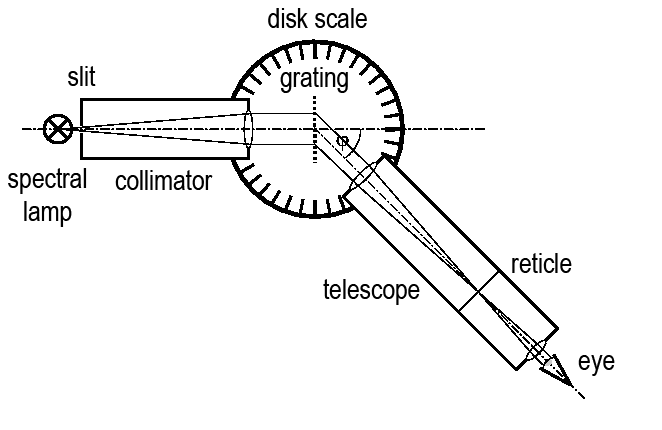
\includegraphics[width=\linewidth/10*6]{images/aufbau}
\caption{Spectrometer design for measuring the spectrum of spectral lamps.\label{aufbau}}
\end{figure}
The following experiment is investigating atomic spectra in the range of visible light. Their origin lies in electronic transisitions with different energies within the atom. A spectrometer is utilized to select the emitted electromagnetic radiation of the assiciated energetic transition. The goal is to understand the design of the spectrometer and test the prediction of the Bohr model on the example of Hydrogen. Additionally, unknown spectral lamps shall be identified with the help of the spectrometer.\\
The experimental setup is shown in fig. (\ref{aufbau}). The metal vapour lamp which is to be analyzed is positioned in front of an adjustable primary slit, which is in the focus of a collective lens, thus creating a beam of parallel light behind it. A line grating scatters the light in all directions, characterized by angle $\varphi$. Since the line grating is parallel to the primary slit we can analyze the diffraction in a plane perpendicluar to the lines.\\
A diffracted beam of parallel light is focussed in the focal plane of a telescope objective/ocular, creating a real image of the primary slit which can by imaged with an appropriate photon detector. The detector used in this experiment is operating on a biophysical principle and you will be provided with two units, both located left and right to your nose\nolinebreak\footnote{Be aware: these detectors are unsuitable for quantitative analysis since their sensitivity is scaled logarithmically. Low intensity profiles will be overestimated compared to the ones with high intensity. The maximum of the sensitivity is around \SI{550}{nm}.}.
The diffraction pattern consists of alternating bright and dark lines parallel to the primary slit. Their frequency and intensity depends on the type of line grating and wavelength of the scattered light.

\subsection{Adjustments to the spectrometer}
The spectrometer is shown in fig. (\ref{spektrometer}). Adjust the telescope (1), slit tube (21) and the stage (22) to a horizontal position by visual judgement. Use the set screws (1.1), (21.1) and (7) to do so. Attach the lighting device (4) to the ocular (3) and turn it on. Focus the reticle in the ocular and align it horizontally, which moves it into the focal plane of the ocular. Focus the telescope on an object aproximately \SI{500}{m} away. It is now focussed on infinite distance.
\begin{figure}[h]
\centering
\includegraphics[width=\linewidth/10*8]{images/spektrometer}
\caption{The spectrometer and accessories (1) telescope; (1.1) set screw for compensating misalignment between telescope (1) and slit tube (21); (2) screw for setting of focus; (3) movable Gaussian ocular; (3.1) opening for light from (4); (4) lighting device; (4.1) locking screw for lighting device; (5) adjustment screw for lateral movement of telescope (1); (6) lockable screw for adjusting height of telescope (1); (7) jackscrew for prism stage (22); locking screw for prism stage (22); (9) locking screw for disc scale; (8) disk scale; (11) fine adjustment for telescope rotation; (12) locking screw for telescope (1); (13) vernier; (14) reading magnifier; (15) height adjustment screw for slit tube (21); (16) adjustment screw for lateral movement of slit tube (21); (17) locking screw for slit pullout; (18) adjustable slit limiter; (19) adjustable slit; (20) micrometer screw for slit opening; (21) slit tube; (21.1) set screw for compensating misalignment between telescope; (22) stage for line grating (23) or prism (24), (23) holder with line grating; (24) holder with prism.\label{spektrometer}}
\end{figure}
For further adjustment you will need a double mirror. Fixate it in the mount for the line grating and position it in the center of the stage, in the way that the connecting line between two of the three verniers is parallel to it. Align the telescope perpendiculary to the mirror. Now bring the mirror image of the reticle to overlap with the reticle itself by compensating half the difference of the horizontal dashes with screw (1.1) and the other half with the vernier screw of the stage table. After that, turn the telescope $180^\circ$ and do the same on the opposite side. Repeat until both dashes are overlapping for both sides. Don't move the stage or mount after this procedure when replacing the double mirror with the line grating now.
It is recommended to position the disk scale in a way that the $0^{th}$ order diffraction reflex is at $0^\circ$. Perform all angular measurements with both verniers to account for possible eccentricity or asymmetry of the disk scale. Measure all spectral lines left and right from the incoming beam. The line grating is tilted and has to be readjusted if the position of the lines varies in height when comparing both sides. For adjusting the line grating parallel to the incoming beam you may use one of the metal vapour lamps. Start with aligning the line grating parallel to the axis of the collimator (by eye measure).
Now place the lamp in front of the primary slit of the collimator, choose a line at a rather high angle, e.g. $>60^\circ$, and identify the angles on both sides. For fine adjustment use the screw (12), therefor the locking screw (11) has to be locked. Calculate the average of both angles and position the telescope to that value. Then turn the stage until this line hits the reticle. Check for the other side as well and repeat if necessary. The adjustment of the line grating is now complete and it should not be moved again.

\subsection{Resolution of the spectrometer}
The Na-lamp works best for demonstrating the resolving capacity of the spectrometer, because the Na-spectrum exhibits two lines in close vicinity. They allow to investigate the influence of the width of the primary slit. Estimate which of the following  parameters has the largest impact on the observed linewidth (see theory section):
\begin{itemize}
\item{intrinsic linewidth}
\item{Doppler broadening}
\item{collision broadening}
\item{resolution of the spectrometer}
\item{width of the primary slit}
\end{itemize}
Approach as follows: Close the primary slit and read the value at micrometer screw (20). Open the primary slit until you can just about distinguish the two lines of the Na-spectrum. You should be able to see multiple diffraction orders for both of them. Note this width setting for the primary slit. Now increase the slit width until both lines start to overlap, also note the value and measure the angular width of the slit image. Assume a linear relationship between the width of the slit and slit image (in $^\circ$) and calculate the resolution limit based on the finite slit size for both Na-lines.

\subsection{lattice constant (line distance) of the line grating}
Any spectral lamp is feasible for this purpose. Choose one and identify the spectrum with the help of table (\ref{TabelleLinien}). Read section \ref{Kapgitter} and calculate the lattice constant $g$ of the line grating. Discuss the intrinsic error. Perform the measurement on both sides of the zero-axis.

\subsection{Measuring the spectrum of the Balmer lamp}
Identify the lines of the Balmer lamp spectrum. Calculate the wavelengths $\lambda_i$ from the measured angles $\varphi_i$ that correspond to the 1$^{st}$ and 2$^{nd}$ order. Estimate the error from the angular measurement and calculate the error in the wavelength using error propagation. Plot $1/\lambda_i$ vs. $1/n_2^2$ and obtain the Rydberg constant from the slope and intersection with the ordinate (see section \ref{KapBohr}). Discuss the error.

\subsection{Measuring the spectrum of an unknown lamp}
Choose a lamp and measure the spectrum. Use table \ref{TabelleLinien} for the identification of the type of lamp.


\begin{table}
\centering
\renewcommand{\arraystretch}{1.2}
\SIobeyboldtrue
\begin{tabular}[htb]{lcccccccccc}\hline\hline
Cadmium&\num{467.8}&\bf{\num{480.0}}&\bf{\num{508.6}}&\num{609.9}&\num{643.8}&&&&&\\
Helium&\num{402.6}&\bf{\num{447.1}}&\num{471.3}&\num{492.2}&\bf{\num{501.6}}&\num{504.8}&\bf{\num{587.6}}&\bf{\num{667.8}}&\num{706.5}&\\
Hydrogen&\num{410.2}&\num{434.0}&\bf{\num{486.1}}&\bf{\num{656.2}}&&&&&&\\
Mercury&\num{404.7}&\bf{\num{435.8}}&\bf{\num{546.1}}&\num{577.0}&\num{579.1}&\num{580.4}&\num{671.6}&\num{690.8}&\num{708.2}&\num{709.2}\\
Neon&\bf{\num{585.2}}&603.0&\bf{\num{618.2}}&\num{626.7}&\bf{\num{640.2}}&\num{650.7}&&&&\\
Sodium&\num{449.8}&\num{568.9}&\num{497.9}&\num{498.3}&\num{568.3}&\num{568.8}&\bf{\num{589.0}}&\bf{\num{589.6}}&\num{615.4}&\num{616.1}\\
Zinc&\num{468.0}&\bf{\num{472.2}}&\bf{\num{481.1}}&\num{518.2}&\bf{\num{636.2}}&&&&&\\ \hline\hline
\end{tabular}
\caption{wavelengths [nm] (in air) of the lines of different spectral lamps in the visible range. The strongest lines are bold.
\label{TabelleLinien}}
\end{table}

\section{Theory}

\subsection{The Bohr atomic model\label{KapBohr}}
In the 19$^{th}$ century scientists were very baffled about the appearance of lines in the spectra of a gas discharge. A famous experiment and its interpretation alongside with a new theory about electromagnetic radiation lead to the breakthrough of its comprehension. Max Planck successfully calculated the intensity of the black body electromagnetic radiation for any wavelength. He postulated therefore that atoms constitute oscillators and that their oscillation energy $E$ is forced to equal discrete evenly spaced values rather than providing a continuous spectrum. Their energy is furthermore proportional to their vibrational frequency $\nu$.
\begin{equation}
E_n=n h \nu\,\,.\label{P1}
\end{equation}
$h$ is Planck's constant and $n$ is an integer. When these oscillators emit energy in the form of electromagnetic radiation it happens in quantified steps from $n$ to $n-1$:
\begin{equation}
\Delta E=E_{n}-E_{n-1}=h\nu\,\,. \label{P2}
\end{equation}

Additionally, in 1911 Ernest Rutherford detected the $\alpha$\,--particle experimentally, when Hans Geiger and Ernest Marsden directed an $\alpha$\,--particle beam onto gold foil and recognizing recoiled specimen. They concluded that the $\alpha$\,--particle consists of an electrically positive core that accounts for almost the full mass of the atom while at the same time sharing a negligible volume fraction of it. This core is surrounded by electrons which show the opposite electronic charge and are thus bound to it by the force of the electrical field. As a whole the atom has no charge. The obvious analogy to the planetary system was revolutionary.\\
These findings were mobilised in 1913 by Niels Bohr in order to explain the electromagnetic spectrum of hydrogen. Following the cosmological analogy the electrons should lose their energy, because accelerated motion leads to the emission of electromagnetic radiation. However, atoms appear to be rather stable and Bohr established postulates in order to circumvent theoretical conflict:
\begin{enumerate}
\item The electron may travel on stationary orbits around the core without losing energy due to the emission of electromagnetic radiation. The orbits are described by equations derived from classical mechanics.
\item The transition from one orbit to another shall be accompanied by the emission of homogeneous electromagnetic radiation. The relationship between the frequency of the emitted radiation and its energy is described by eq. (\ref{P2}).
\end{enumerate}
The binding energy $E$ of an electron with the reduced mass $m_e$, charge $e$ and velocity $v$ on such a classical orbit is
\begin{equation}
E=\frac{1}{2 r}\left(\frac{e^2}{4 \pi \epsilon_0}\right)\label{B1}
\end{equation}
and is equal to the kinetic energy.
$e$ is the elementary charge, $\epsilon_0$ the dielectric constant and $r$ the radius of the orbit. Equilibrium of forces states that
\begin{equation}
r=\left(\frac{e^2}{4 \pi \epsilon_0}\right)\frac{1}{m v^2}\,\,.\label{B2}
\end{equation}

$m=m_e\,m_p/(m_e+m_p)$ ($m_p$: proton mass) is the $reduced$ $mass$.
For the rotational frequency $f$ one obtains
\begin{equation}
f=\left(\frac{4 \pi \epsilon_0}{e^2}\right)\sqrt{\frac{2}{m}}\,\frac{E^{3/2}}{\pi}\,\,.\label{B3}
\end{equation}
Bohr attributed to the stationary orbits that
\begin{equation}
E_n=n\, h\, \frac{f}{2}\,\,.\label{B4}
\end{equation}
With equation (\ref{B3}) one obtains the energy for the orbits
\begin{equation}
E=E_n=\left(\frac{e^2}{4 \pi \epsilon_0}\right)^2\frac{2 \pi^2 m}{h^2 n^2}\,\,.\label{B5}
\end{equation}
From the second postulate it follows that energy $\Delta E$ and frequency $\nu$ of the emitted waves
\begin{equation}
\Delta E=E_{n_1}-E_{n_2}=h\nu=\left(\frac{e^2}{4 \pi \epsilon_0}\right)^2\frac{2 \pi^2 m}{h^2}
\,\,\left(\frac{1}{n_1^2}-\frac{1}{n_2^2}\right)\,\,.\label{B6}
\end{equation}
With the relation $\lambda=c/\nu$ one obtains for the wavelength $\lambda$ of the emitted radiation ($c$ : speed of light)
\begin{equation}
\frac{1}{\lambda}=R\left(\frac{1}{n_1^2}-\frac{1}{n_2^2}\right)\,\,.\label{B7}
\end{equation}
$R=\left(\frac{e^2}{4 \pi^2 \epsilon_0}\right)^2\frac{2 \pi m}{h^3 c}=\SI{1.097e7}{m^{-1}}$ is the Rydberg constant. 1885 Jakob Balmer already empirically confirmed eq. (\ref{B7}) for $n_1=2$ and
$n_2>2$ for wavelengths in the visible range of light.

Eqs. (\ref{B1}) to (\ref{B7}) remain valid for ions that are structurally similar to hydrogen, such as He$^+$, Li$^{2+}$, Be$^{3+}$, when one replaces $e^2 \longrightarrow Z\,e^2$. $Z$  is the core charge of the ion.
The simple analogy of the hydrogen atom to the planety system was proven wrong by quantum mechanics in the 20$^{th}$ century. However, the energetic levels found by Bohr are nevertheless correctly described for hydrogen. But already for the Helium atom it is not possible to find such easy analytical expressions. The reason for that is electron-electron interaction which is neglected in the Bohr atomic model. Such a system can only be understood by solving Schroedingers equation to obtain the energetic states of the electrons. If you know these, you can then relate their energy to the frequency of the emitted electromagnetic radiation with relation $\Delta E=E_1-E_2=h\nu$, where the electron transitions from state 1 to 2 with energies $E_1$ and $E_2$, respectively.
The state of an electron within an arbitrary atom is generally characterized by a set of parameters. The transition of one state to another can be restricted by selection rules. Within the scope of this experiment, however, we limit ourselves to use classical atomic physics. 

\subsection{Spectral linewidth}
The Bohr atomic model allows us to calculate the position of the lines in the hydrogen spectrum, but gives no information about their width. The intrinsic spectral linewidth can be estimated by the life span of an excited state using the uncertainty principle [Heisenberg].
\begin{equation}
\delta E \,\delta t \geq \hbar \label{Heisenberg}
\end{equation}
$\Delta E$ is the width of the line and $\Delta t$ the life span of the state. A typical value is \SI{e-8}{s}. One is now able to estimate the length of the emitted wave packet.
Due to atomic motion (at ambient temperature typically some hundert meters per second, accordingly more in a spectral lamp) the wavelength of the emitted radiation is shifted towards smaller or larger values due to the Doppler effect. This leads to an additional broadening of the spectral lines. The half width $\Delta E_D$ of the Doppler broadening for a line with frequency $\nu_0$ (see e.g. \reference{Ott93}):
\begin{alignat}{2}
\label{Doppler}
&\qquad\qquad M &\quad&\text{atomic mass}\nonumber\\
\frac{\delta E_{Doppler}}{h\nu}=\frac{2}{c}\sqrt{\frac{2kT}{M}\ln 2}\,\,. &\qquad\qquad k 
&&\textrm{Boltzmann constant}\\
&\qquad\qquad T &&\text{temperature}\nonumber
\end{alignat}
Apart from the Doppler effect there is broading due to collision of atoms. When a radiation emitting atom collides with another one, usually the polarization, direction and/or duration of the emission is affected. These scattering events contribute to the linebroadening. If one assumes that the time between two collisions is longer than the collision itself, but shorter than average life span of an excited state, one can formulate for the half maximum for the resulting distribution (see e.g. \reference{Ott93}):
\begin{alignat}{2}
\label{Stoss}
&\qquad\qquad n &\quad&\text{atomic density of the gas}\nonumber\\
\frac{\delta E_{coll}}{2}=h\,n\,\sigma\,\overline{v}\,\,.&\qquad\qquad \sigma&&\text{cross section for elastic scattering}\\
&\qquad\qquad \overline{v}&&\text{average atomic velocity}\nonumber
\end{alignat}
The scattering cross section can be estimated by $\sigma=\pi a_0^2$, where $a_0=\SI{0.53}{\text{\AA}}$ is the Bohr radius.
For the average velocity it holds:
\begin{equation}
\bar{v}=\sqrt{\frac{8\,k\,T}{\pi\,M}}\,\,\label{mittG}.
\end{equation}

\subsection{The physics behind the line grating\label{Kapgitter}}
We use a transmissible line grating to separate different wavelengths. The optical path is illustrated in fig. (\ref{gitter}). A plane wave approaches the grating from the left. wave crests and troughs are visualised with thick and thin lines, respectively. The grating is a collection of parallel slits with uniform distance $g$ and in this geometry they can be treated as infinitesimal thin and infinitely long. The grating disturbs the homogeneous wave and diffracts it.
\begin{figure}[htb]
\centering
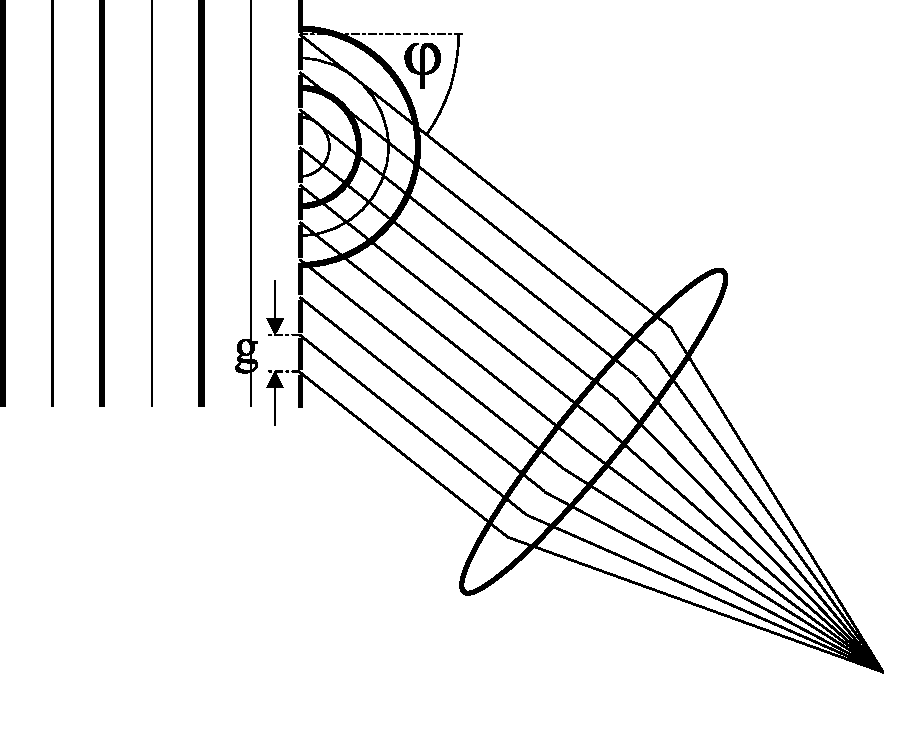
\includegraphics[width=\linewidth/10*5,clip]{images/gitter}
\caption{Fraunhofer diffraction at the grating.\label{gitter}}
\end{figure}
Following Huygens principle, every point in the wave can be seen as source of a new spherical wave. Such a wave is shown in fig. (\ref{gitter}) for a single slit. When aligning the grating perpendicularly to the incoming parallel wave, all spherical waves have the same phase and amplitude. Thanks to the inherent symmetry we can treat the scenario from the simplified perspective of a plane that is orthogonal to the grating plane. The transmitted wave is a result of superposition of all the spherical waves from each slit.
If you look at the emitted spherical wave from a distance that is much larger than the width of the slit you can approximate it as a plane wave, as it is visualised in fig. (\ref{gitter}) by lines (beams) that are perpendicular to the wavefront.
The phase difference $\delta$ of two these beams with the wavelength $\lambda$ going in a direction defined by $\varphi$ are
\begin{equation}
\delta=2 \pi \frac{g \sin{\varphi}}{\lambda}  \label{delta}
\end{equation}
Focussing all beams through a lens it is the phase that decides whether combined intensity cancels (partly) or is enhanced. The lens will not alter the phase by keeping the optical paths the same for all beams.
A wave that propagates in $x$-direction can be expressed as the real part of a complex exponential function:
\begin{equation}
E=A\cos{\left(2\pi\nu(t-x/c)\right)}=A\,\Re\left\{\eu{\,i[2\pi\nu(t-x/c)]}\right\} \,\,.
\end{equation}
For $p$ beams that have a phase shift of $\delta$ each one obtains
\begin{eqnarray}
E_1&=&A\,\Re\left\{\,\eu{\,i[2\pi\nu(t-x/c)]}\right\}\\
E_2&=&A\,\Re\left\{\,\eu{\,i[2\pi\nu(t-x/c)-\delta]}\right\}\\
\vdots\\
E_p&=&A\,\Re\left\{\,\eu{\,i[2\pi\nu(t-x/c)-(p-1)\delta]}\right\}\,\,.
\end{eqnarray}
The strength of the electrical field $E=E_1+E_2+\dots+E_p$ is thus
\begin{equation}
E=A\,\Re\left\{\,\eu{\,i2\pi\nu(t-x/c)}\right\}\left[1+\eu{\,-i\delta}+\dots+
\eu{-i(p-1)\delta}\right]\,\,.      \label{Esumme}
\end{equation}
For the geometric series in the brackets it holds that
\begin{equation}
\left[1+\eu{\,-i\delta}+\dots+
\eu{-i(p-1)\delta}\right]=\frac{1-\eu{-i p \delta}}{1-\eu{-i\delta}}\,\,.\label{georeihe}
\end{equation}
If you insert eq. (\ref{georeihe}) in eq. (\ref{Esumme}) and calculate the real part one obtains
\begin{equation}
E=A\,\frac{\sin(p\,\delta/2)}{\sin(\delta/2)}\cos\left[2\pi\nu(t-x/c)-(p-1)\,\delta/2\right]\,\,.
\end{equation}
The intensity is the time average of the field squared
\begin{equation}
I=A^2/2\,\frac{\sin^2(p\,\delta/2)}{\sin^2(\delta/2)}\,\,.\label{Intensity}
\end{equation}
\begin{figure}[ht]
\centering
\includegraphics[width=\linewidth/10*5,clip]{images/multipleinterference}
\caption{Intensity distribution of a grating following eq. (\ref{Intensity}).
\label{multipleinterference}}
\end{figure}
This function is shown in fig. (\ref{multipleinterference}). The main maxima are located where the denominator equals zero, i.e. $\delta/2=n\pi$, $n=\pm 1,\pm 2, \dots\,\,$. In between one will find $p-2$ local maxima when the enumerator is zero. The intensity of the main maxima scales with $p^2$ and their width is increasing with the number $p$ of interferent beams. The local maxima are fading with $p$.\\
Using  eq. (\ref{delta}) for the value of $\delta$ one obtains the position of the main maxima
\begin{equation}
\frac{g \sin{\varphi}}{\lambda}=n\,, \,\,n=\pm 1,\pm 2, \dots\,\,.  \label{lagemax}
\end{equation}
The number $n$ is the order of the diffraction reflex. With known $g$ and given $\varphi$ one can calculate the wavelength. Conversively one can determine $g$ when knowing the wavelength.
If one assumes a finite size $b$ of the slits, the pattern will change only minimally. The position of the maxima will remain the same. A calculation shows that eq. (\ref{Intensity}) is modulated with the intensity profile of a single slit then. The intensity will be
\begin{equation}
I=A^2/2\,\frac{\sin^2(\tilde{\delta}/2)}{(\tilde{\delta}/2)^2}\,
\frac{\sin^2(p\,\delta/2)}{\sin^2(\delta/2)}\,\,.\label{Intensity2}
\end{equation}
$\tilde{\delta}$ is obtained by replacing $g\rightarrow b$ in eq. (\ref{delta}).
\begin{figure}[hb]
\centering
\includegraphics[width=\linewidth/10*5]{images/finiteslitsize}
\caption{Intensity profile of the grating with a finite slit width $b$.
\label{finiteslitsize}}
\end{figure}
For the case $g/b=3$ eq. (\ref{Intensity2}) is shown in fig. (\ref{finiteslitsize}).
If the grating is tilted by $\varphi_0$ against the wavefronts, eq. (\ref{lagemax}) has to be replaced by the following
\begin{align}
\sin(\varphi_l-\varphi_0)+\sin(\varphi_0)&=\frac{n}{g}\lambda \nonumber\\
\sin(\varphi_r+\varphi_0)-\sin(\varphi_0)&=\frac{n}{g}\lambda\,\,.
\end{align}
$\varphi_l$ and $\varphi_r$ are the angles left and right from the collimator axis, respectively.
With $\sin(\alpha+\beta)=\sin(\alpha)\cos(\beta)+\cos(\alpha)\sin(\beta)$ and the small angle approximation $\cos(\varphi_0)=1$ und $\sin(\varphi_0)=\varphi_0$ one obtains from the summation of these two equations
\begin{equation}
\sin(\varphi_l)+\sin(\varphi_r)+\varphi_0\left(\cos(\varphi_l)-\cos(\varphi_r)\right)=\frac{2\,n}{g}\lambda\,\,.\label{lage2}
\end{equation}
The third expression on the left side can be neglected for small $\varphi_0$.
Eq. (\ref{lage2}) demonstrates, that in the case of an offset in the line position relative to the zero-degree axis the sine of the angles has to be averaged, not the angles themselves.


\subsection{Resolution}
The resolution $R$ of the spectrometer quantifies its ability to seperate the locations of two lines that vary in the wavelength by $\delta \lambda$. It is defined as
$R=\lambda /\delta \lambda$.
\begin{figure}[htb]
\centering
\includegraphics[width=\linewidth/10*5,clip]{images/auflverm}
\caption{Resolution of a grating with $p=900$ interfering beams of the Na-double line.
\label{AuflVerm}}
\end{figure}
Fig. (\ref{AuflVerm}) shows the intensity profile of two lines with the wavelengths $\lambda$ and $\lambda+\delta\lambda$. The total intensity is a superposition of the single intensities since one can assume that in general all lines are incoherent. A distinction of the lines is possible if their half widths are on the verge of overlapping, leaving a small visible saddle point.
The half width of profile (\ref{Intensity}) as a function of $\delta$ is equal to $\delta_{1/2}=\num{2.783}/p$. As a function of $\varphi$ it is $\varphi_{1/2}=\num{2.783}\tan(\varphi)/(p\pi n)$. With eq. (\ref{lagemax}) it follows that
\begin{equation}
R=\frac{\lambda}{\left|\dquot{\lambda}{\varphi}\right|\diff\varphi}=\num{1.129}\,np\,\,.\label{Aufl}
\end{equation}
A higher order $n$ and a larger number of interfering beams guarantees an improving resolution.
Eq. (\ref{Aufl}) is valid only with the absence of aberrations and an infinitesimal narrow primary slit. Since the primary slit is focussed in the focal plane of the telescope, see fig. (\ref{aufbau}), the line width will always be finite (even with $p=\infty$) and larger than calculated with eq. (\ref{Aufl}).


\frage{How much different is the wavelength of visible light in air when compared to vacuum?
(Hint: $c_{vac}/c_{air}=\num{1.0003}$)}

\frage{Derive eq. (\ref{B7}) by postulating that the angular momentum $l$ is an integer of $l_0=h/2\pi$.}

\frage{Search for He lines in table (\ref{TabelleLinien}) that are in accordance with eq. (\ref{B7}) and the substitution $e^2 \rightarrow Z\,e^2$ ($Z=2$ for He)?}

\frage{What is the effect on the wavelength if we record a deuterium (mass: \SI{2}{u}) spectrum instead of hydrogen (mass: \SI{1}{u})?}

\frage{calculate the energy and wavelengths of photons that are emitted from an electronic transition $n_2=3,4,5,6$ to $n_1=2$. Repeat the calculations for the case $n_2=4,5,6$ to $n_1=3$. Which of these transitions are visible?}

\frage{What is the error you get when the grating is tilted against the incoming plane wave propagation direction by the angle $\varphi_0=\num{0.3}^\circ$? Neglect the third term on the left side of eq. (\ref{lage2}).}

\end{document}
